\documentclass[a4paper, 12pt]{article}

\usepackage{geometry}
\usepackage{amsmath}
\usepackage{gvv}

\title{Question 4.8.36}
\author{AI25BTECH11040 - Vivaan Parashar}
\date{\today}

\begin{document}

\maketitle

\section{Question: }
Find the equation of the plane determined by the points $\vec{A}$(3, -1, 2), $\vec{B}$(5, 2, 4) and $\vec{C}$(-1, -1, 6). Also find the distance of the point $\vec{P}$(6, 5, 9) from the plane.

\section{Solution: }
A plane in 3D is represented by the equation $\vec{n}^\mathrm{T}\vec{x} = c$, where the vector $\vec{n}$ represents the normal to the plane, and $c$ is an arbitrary constant, that can be set to $1$ for simplicity.
We have three points that lie on the plane, $\vec{A}$, $\vec{B}$, and $\vec{C}$. We therefore have the following equations:
\begin{align}
    \vec{n}^\mathrm{T}\vec{A} = 1\\
    \vec{n}^\mathrm{T}\vec{B} = 1\\
    \vec{n}^\mathrm{T}\vec{C} = 1\\
    \implies\vec{n}^\mathrm{T}\myvec{\vec{A} & \vec{B} & \vec{C}} = \myvec{1 & 1 & 1}\\
\end{align}
Let's call the matrix $\myvec{\vec{A} & \vec{B} & \vec{C}}$ $\vec{M}$. Multiply both sides by $\vec{M}^\mathrm{-1}$ on the right:
\begin{align}
    \therefore \vec{n}^\mathrm{T} = \myvec{1 & 1 & 1}\vec{M}^\mathrm{-1} = \myvec{1 & 1 & 1}\myvec{3 & 5 & -1 \\ -1 & 2 & -1 \\ 2 & 4 & 6}^\mathrm{-1}\\
    \implies \vec{n}^\mathrm{T} = \frac{1}{19}\myvec{3 & -4 & 3}
\end{align}
Thus, the equation of the plane is given by:
\begin{align}
    \myvec{3 & -4 & 3}\vec{x} = 19
\end{align}
The distance $d$ of the point $\vec{P}$ from the plane is given by:
\begin{align}
    d = \frac{|\vec{n}^\mathrm{T}\vec{x_P} - c|}{\|\vec{n}\|}\\
    \implies d = \frac{|\myvec{3 & -4 & 3}\myvec{6 \\ 5 \\ 9} - 19|}{\sqrt{(3)^2 + (-4)^2 + (3)^2}}\\
    \implies d = \frac{6}{\sqrt{34}}
\end{align}

\section{Plot: }
\begin{figure}[h!]
    \centering
    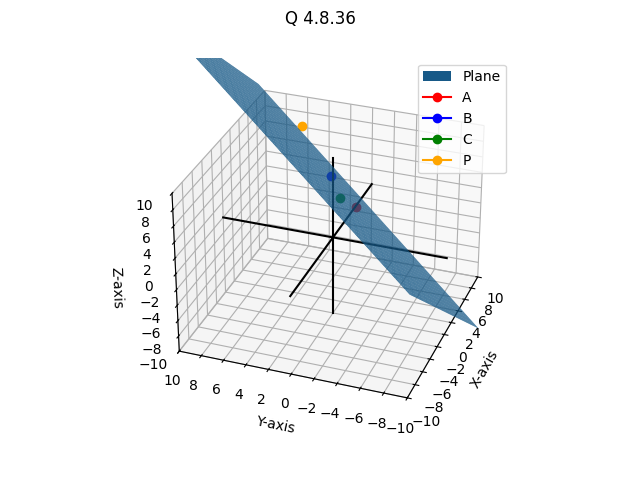
\includegraphics[width=\columnwidth]{figs/plot.png}
    \caption{Graph of plane and points A, B, C and P}
    \label{fig:4.2.3}
\end{figure}


\end{document}